% Options for packages loaded elsewhere
\PassOptionsToPackage{unicode}{hyperref}
\PassOptionsToPackage{hyphens}{url}
%
\documentclass[
  11pt,
]{article}
\usepackage{amsmath,amssymb}
\usepackage{lmodern}
\usepackage{ifxetex,ifluatex}
\ifnum 0\ifxetex 1\fi\ifluatex 1\fi=0 % if pdftex
  \usepackage[T1]{fontenc}
  \usepackage[utf8]{inputenc}
  \usepackage{textcomp} % provide euro and other symbols
\else % if luatex or xetex
  \usepackage{unicode-math}
  \defaultfontfeatures{Scale=MatchLowercase}
  \defaultfontfeatures[\rmfamily]{Ligatures=TeX,Scale=1}
\fi
% Use upquote if available, for straight quotes in verbatim environments
\IfFileExists{upquote.sty}{\usepackage{upquote}}{}
\IfFileExists{microtype.sty}{% use microtype if available
  \usepackage[]{microtype}
  \UseMicrotypeSet[protrusion]{basicmath} % disable protrusion for tt fonts
}{}
\makeatletter
\@ifundefined{KOMAClassName}{% if non-KOMA class
  \IfFileExists{parskip.sty}{%
    \usepackage{parskip}
  }{% else
    \setlength{\parindent}{0pt}
    \setlength{\parskip}{6pt plus 2pt minus 1pt}}
}{% if KOMA class
  \KOMAoptions{parskip=half}}
\makeatother
\usepackage{xcolor}
\IfFileExists{xurl.sty}{\usepackage{xurl}}{} % add URL line breaks if available
\IfFileExists{bookmark.sty}{\usepackage{bookmark}}{\usepackage{hyperref}}
\hypersetup{
  hidelinks,
  pdfcreator={LaTeX via pandoc}}
\urlstyle{same} % disable monospaced font for URLs
\usepackage[margin=1in]{geometry}
\usepackage{longtable,booktabs,array}
\usepackage{calc} % for calculating minipage widths
% Correct order of tables after \paragraph or \subparagraph
\usepackage{etoolbox}
\makeatletter
\patchcmd\longtable{\par}{\if@noskipsec\mbox{}\fi\par}{}{}
\makeatother
% Allow footnotes in longtable head/foot
\IfFileExists{footnotehyper.sty}{\usepackage{footnotehyper}}{\usepackage{footnote}}
\makesavenoteenv{longtable}
\usepackage{graphicx}
\makeatletter
\def\maxwidth{\ifdim\Gin@nat@width>\linewidth\linewidth\else\Gin@nat@width\fi}
\def\maxheight{\ifdim\Gin@nat@height>\textheight\textheight\else\Gin@nat@height\fi}
\makeatother
% Scale images if necessary, so that they will not overflow the page
% margins by default, and it is still possible to overwrite the defaults
% using explicit options in \includegraphics[width, height, ...]{}
\setkeys{Gin}{width=\maxwidth,height=\maxheight,keepaspectratio}
% Set default figure placement to htbp
\makeatletter
\def\fps@figure{htbp}
\makeatother
\setlength{\emergencystretch}{3em} % prevent overfull lines
\providecommand{\tightlist}{%
  \setlength{\itemsep}{0pt}\setlength{\parskip}{0pt}}
\setcounter{secnumdepth}{-\maxdimen} % remove section numbering
\usepackage{subfig} \usepackage{fancyhdr} \thispagestyle{empty} \usepackage{titling} \pretitle{\centering \vspace*{-1cm}\hspace*{-1cm}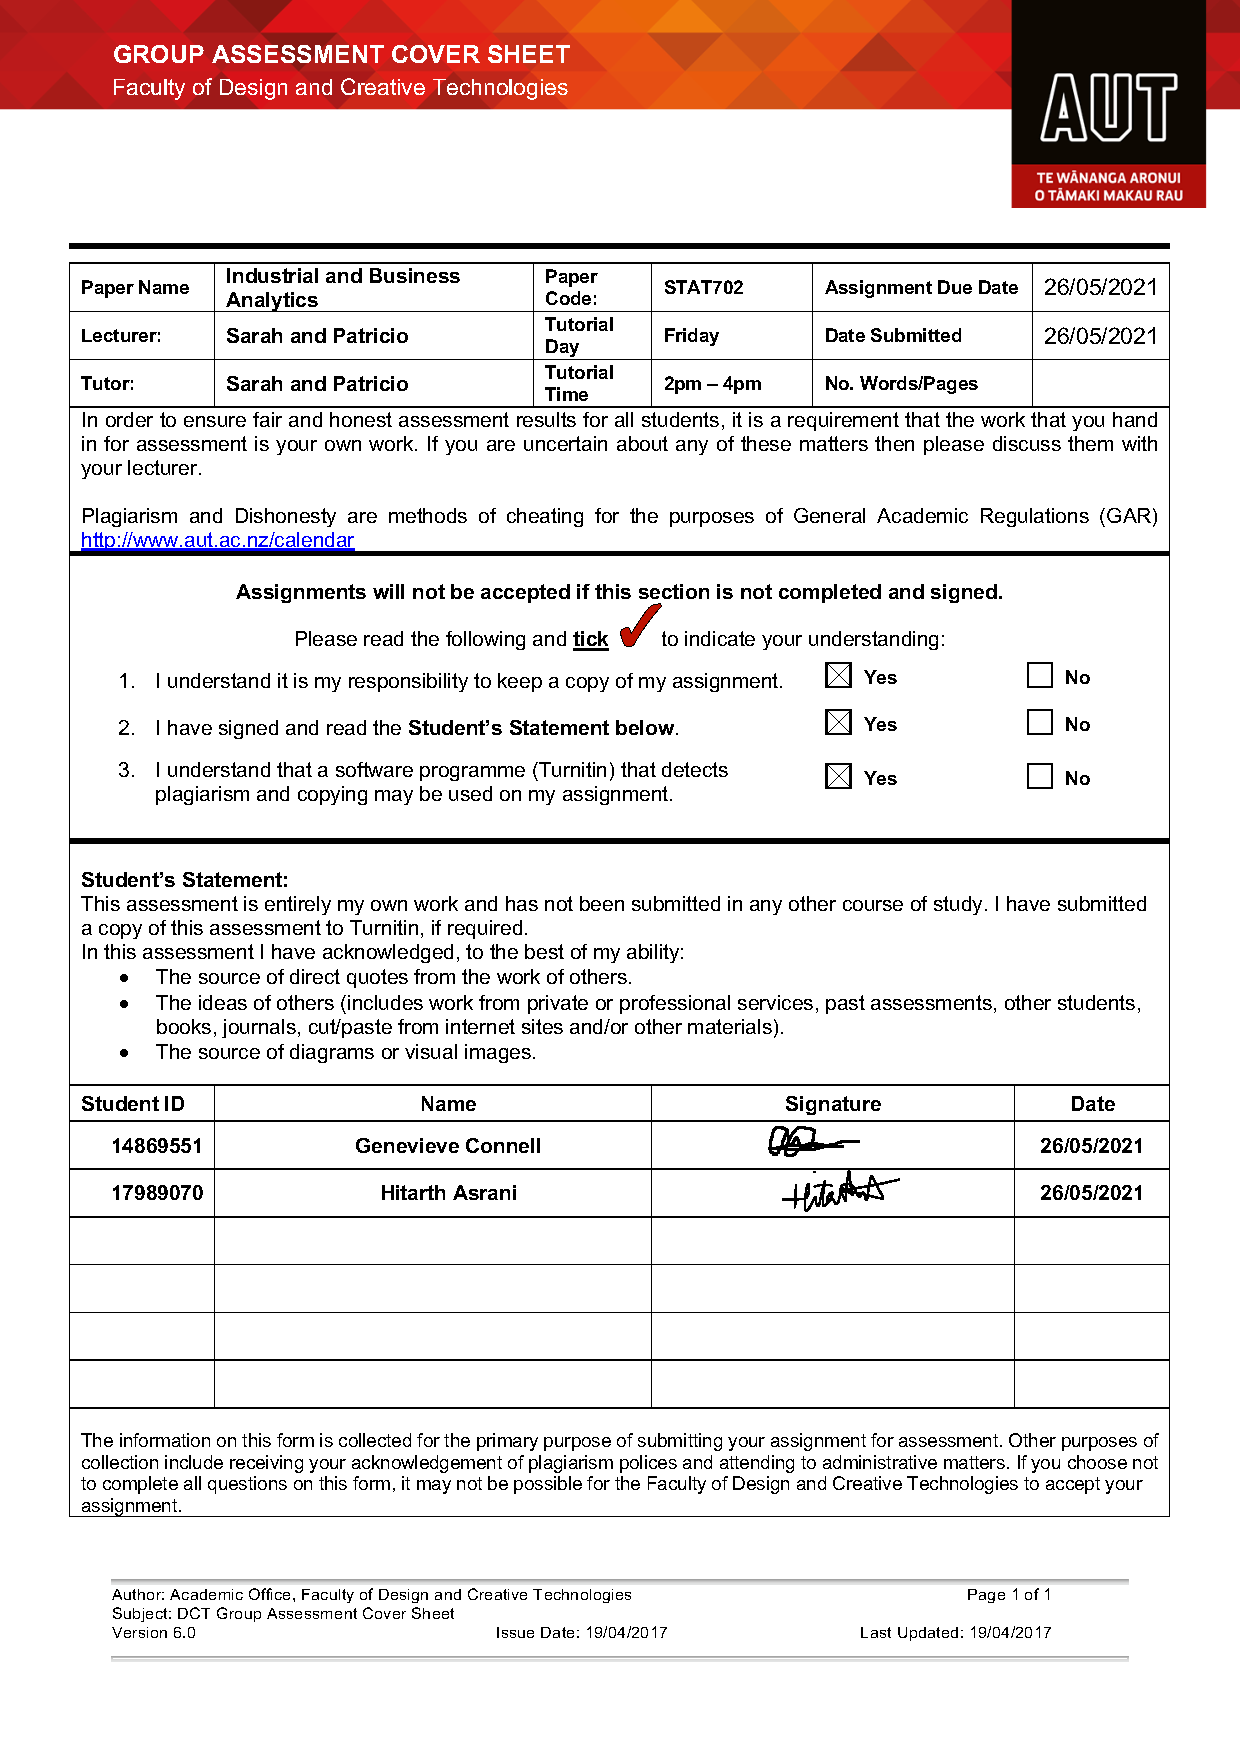
\includegraphics[width=15.5cm]{DCT-Group-Assessment-Cover-Sheet.pdf} \\[\bigskipamount] \newpage    \vspace*{3cm} \begin{center} \bf \LARGE} \posttitle{\end{center}  } \pagestyle{fancy} \fancyhf{} \renewcommand{\headrulewidth}{0pt} \fancyfoot[LE,RO]{\thepage}
\usepackage{float}
\ifluatex
  \usepackage{selnolig}  % disable illegal ligatures
\fi

\title{STAT702 Industrial and Business Analytics\\
Project}
\author{Genevieve Connell and Hitarth Asrani}
\date{26 May 2021}

\begin{document}
\maketitle

\newpage

\hypertarget{analysis-of-sales-data}{%
\section{1. Analysis of Sales Data}\label{analysis-of-sales-data}}

\textbf{Product name}: BIC Round Stic Xtra Life Ballpoint Pen, Medium
Point (1.0mm), Red, 12-Count

\textbf{Sales sku\_id}: 219884

\textbf{Reviews asin}: B00006IE7J

\hypertarget{a}{%
\subsection{1.a}\label{a}}

From Jan 2011 - July 2013, 98434 units of sku 219844 were sold with a
monthly mean of 3175.3. In the plots below monthly sales do not appear
to follow a trend or seasonal pattern. Three months stand out with high
sales, these are May 2011, December 2011 and January 2012. The most
significant high sales occurred in January 2012 when 8871 units were
sold. As shown in the plots below these high monthly sales correspond
with a high proportion of stores featuring and/or displaying the
product, resulting in unusually high sales.

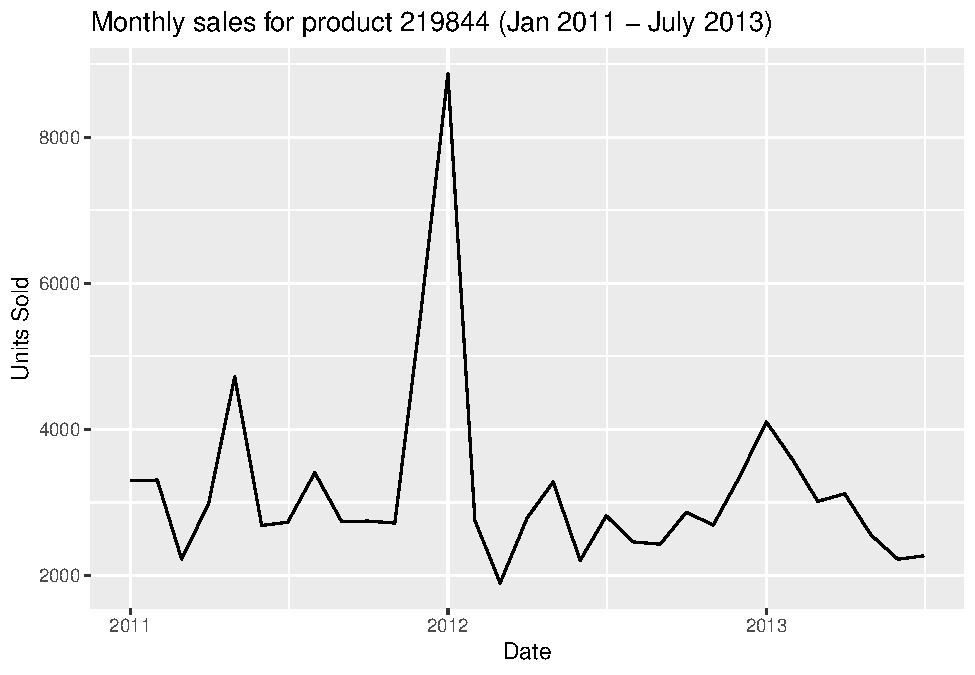
\includegraphics[width=0.6\linewidth]{Assignment-STAT702---final_files/figure-latex/1a monthly sales plot-1}

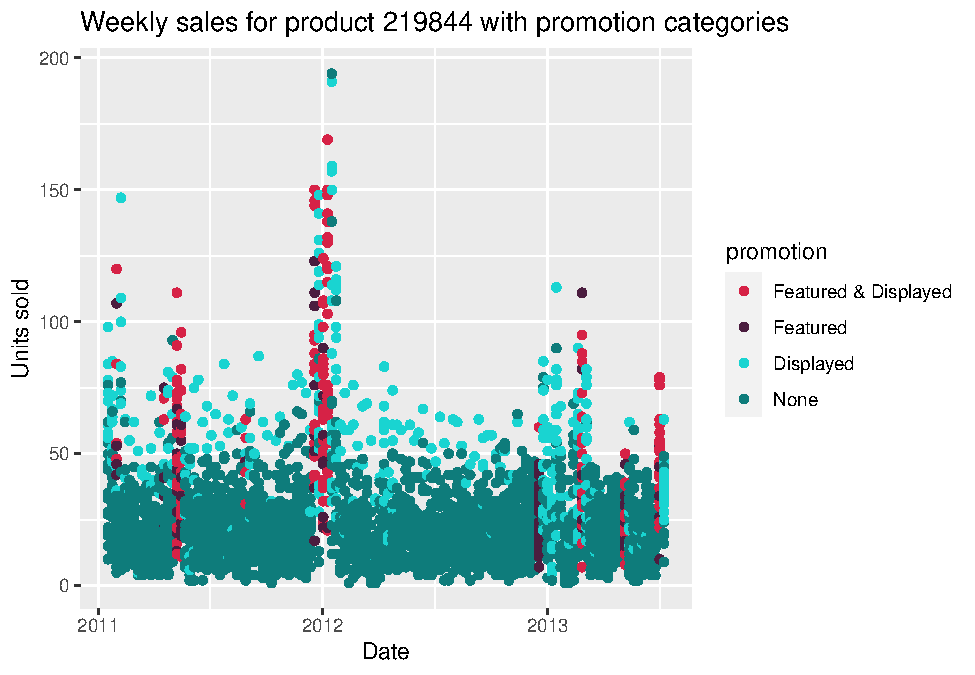
\includegraphics[width=0.5\linewidth]{Assignment-STAT702---final_files/figure-latex/test, figures-side-1}
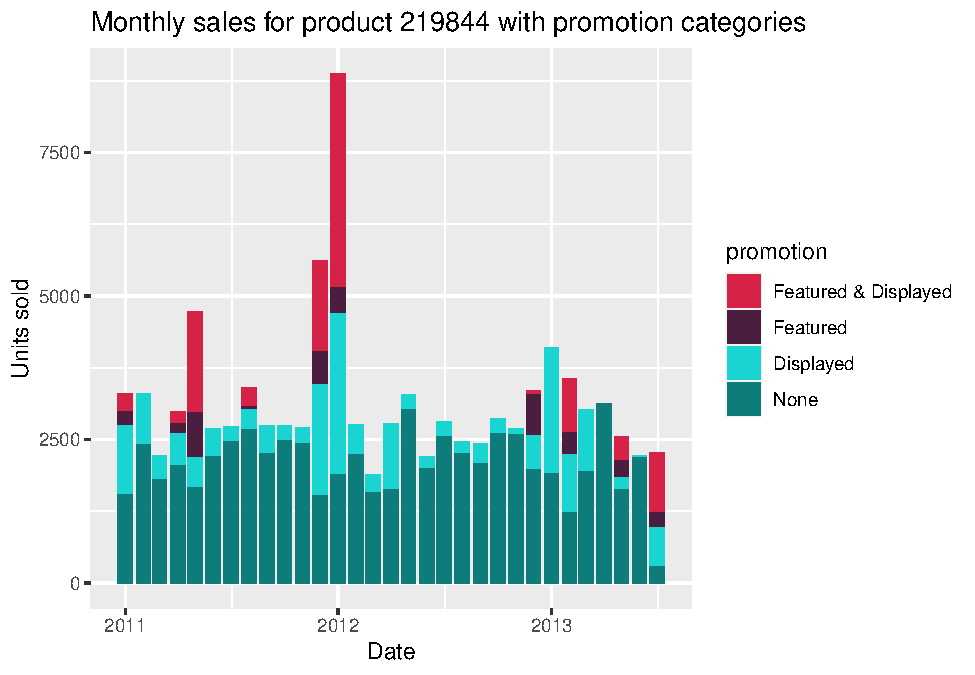
\includegraphics[width=0.5\linewidth]{Assignment-STAT702---final_files/figure-latex/test, figures-side-2}

\hypertarget{b}{%
\subsection{1.b}\label{b}}

All stores have been ranked based on their total sales from Jan 2011 to
July 2013. The store with the highest total units sold is ranked `1',
this is store 9279 with 6698 units. Below is a bar chart showing the
total units sold with stores ordered by rank. Sales for 2013 are much
lower than 2011 and 2012 as only half the years data is included.

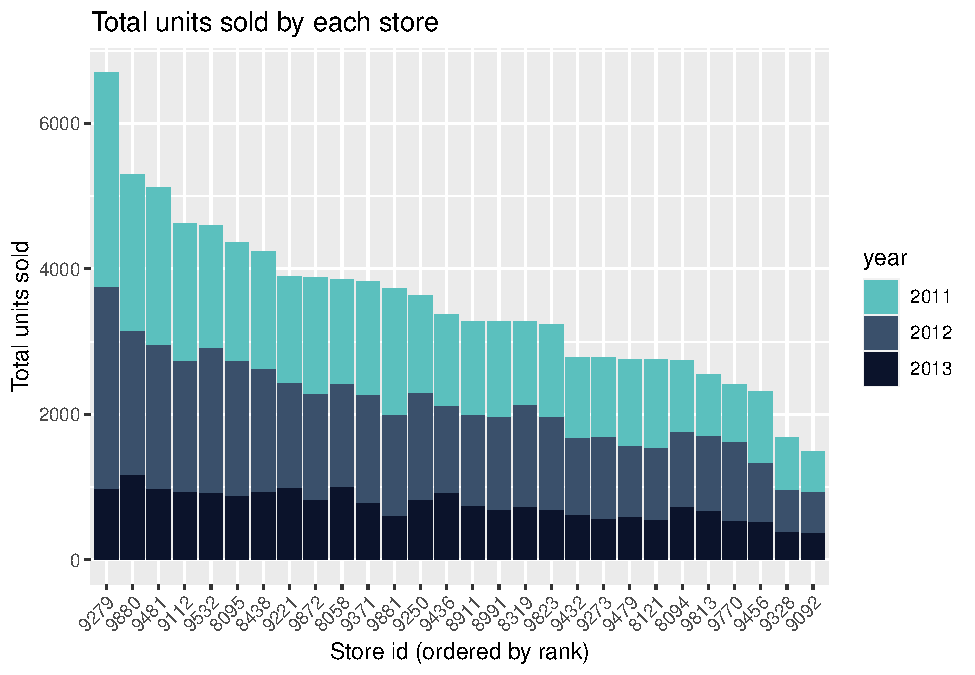
\includegraphics[width=0.75\linewidth]{Assignment-STAT702---final_files/figure-latex/1b store totals plotted-1}

For a more detailed look at store performance monthly sales have been
plotted for each store and categorised as `High', `Average' or `Low'
performing. These categories are based on the interquartile range for
monthly sales. This range is 71 - 138 and captures 50\% of all monthly
sales. Monthly sales within the range are classified as `Average', sales
greater than 138 are classified as `High' performing and those below 71
are classified as `Low' performing. Summary statistics for store monthly
sales are below.

\begin{longtable}[]{@{}llllll@{}}
\toprule
Min & 1st Qu. & Median & Mean & 3rd Qu. & Max \\
\midrule
\endhead
19 & 71 & 95.5 & 113.4 & 138 & 571 \\
\bottomrule
\end{longtable}

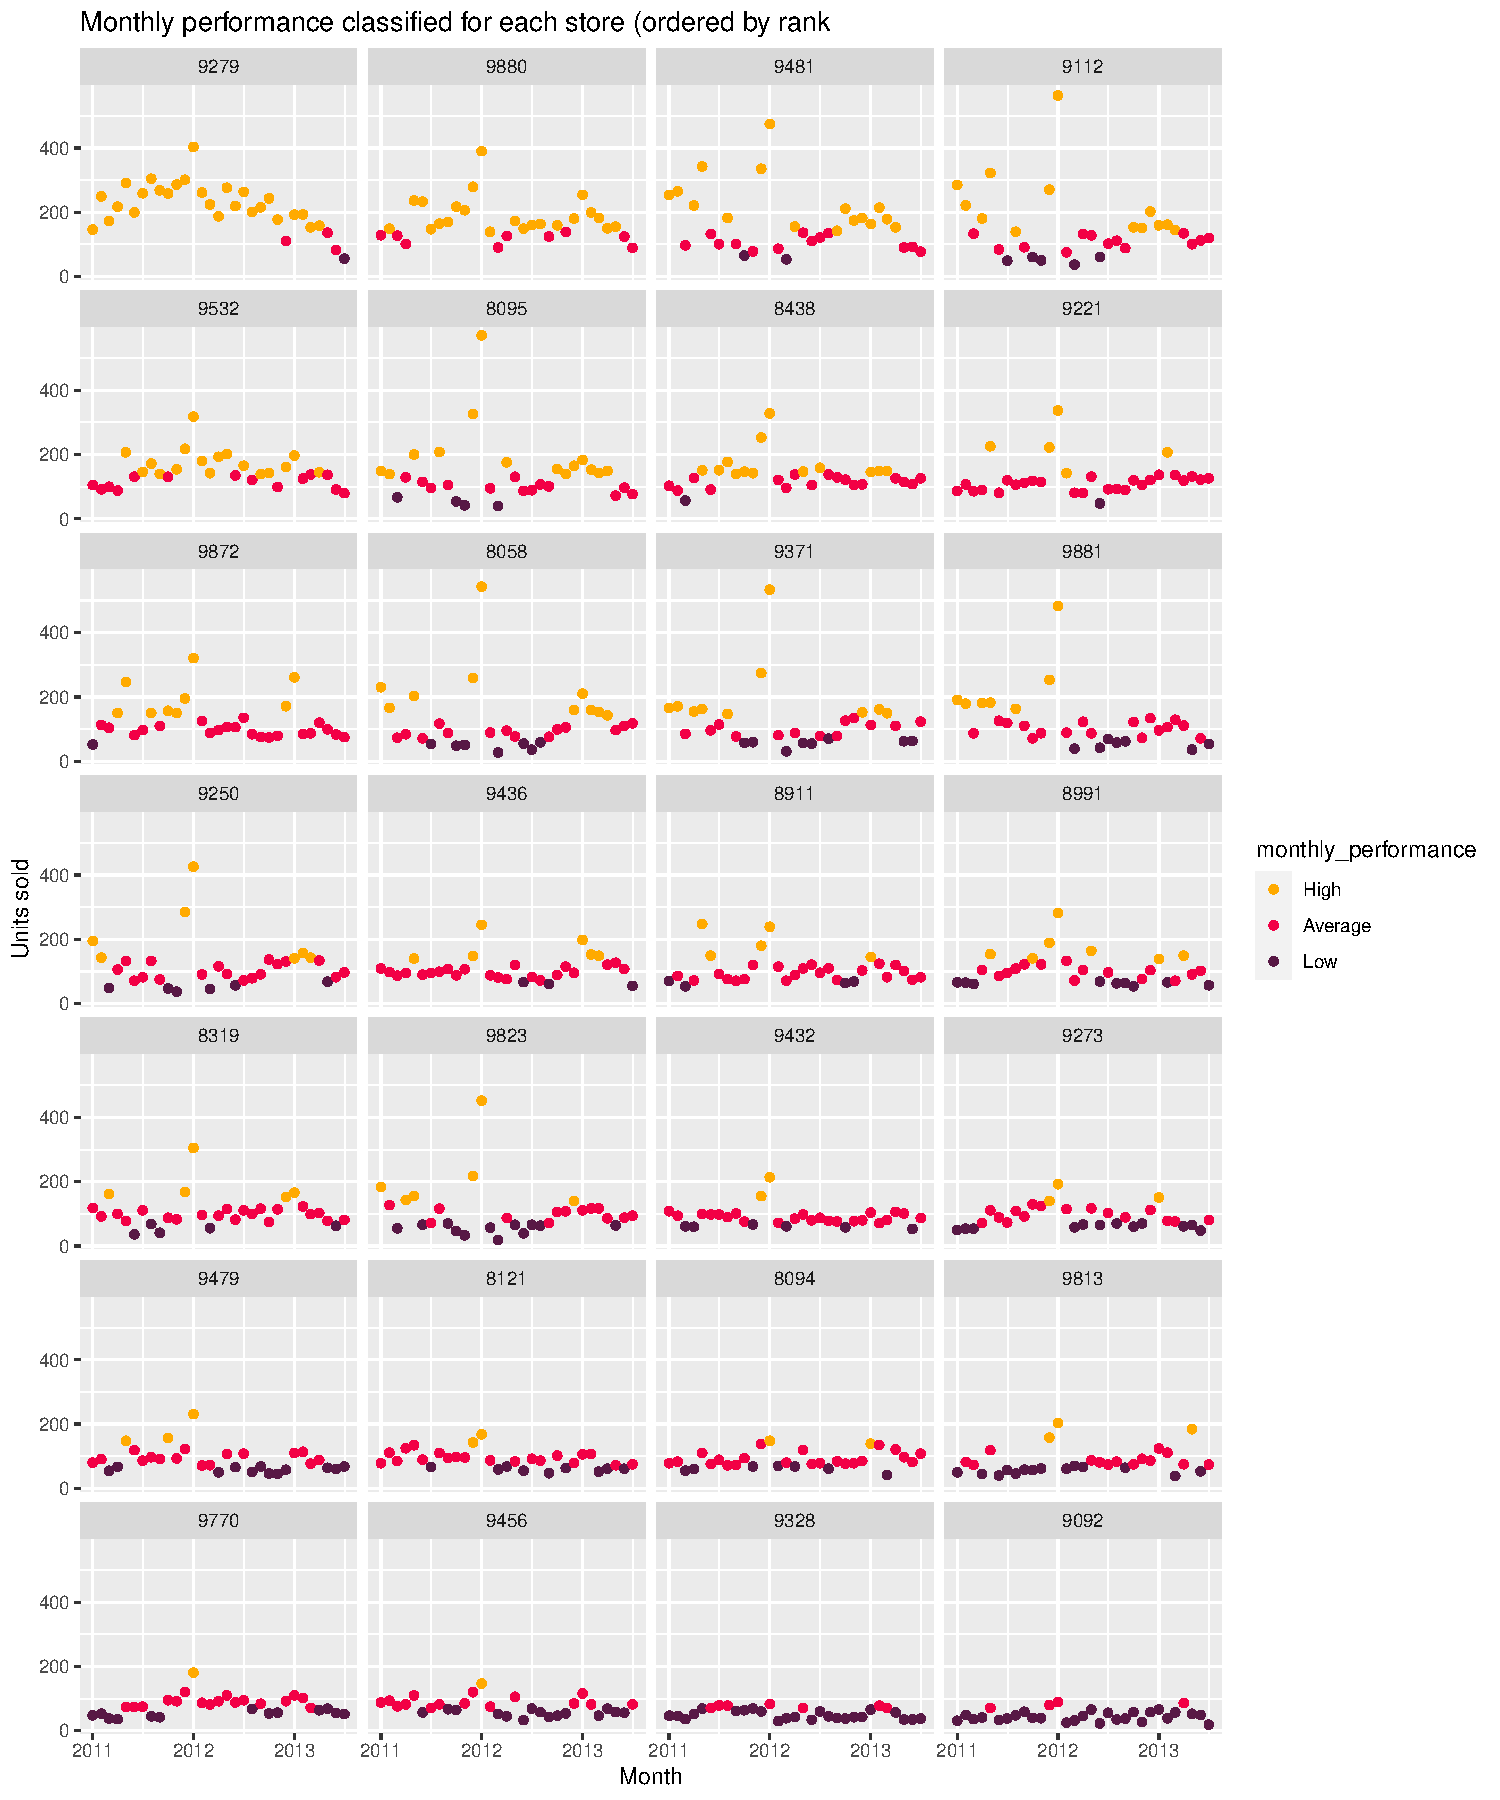
\includegraphics{Assignment-STAT702---final_files/figure-latex/store plots-1.pdf}
An interesting feature of these plots is that some stores have more
consistent performance than others. For example store 9112 had 5 low
performing months but was ranked at 4, much higher than store 9872 which
had only 1 low performing month but was ranked 9. Stores with high
occurrences of low sales are not reliable and are a source of risk to an
organisation.

As an alternative to ranking stores based on their overall sales, stores
have been given a ranking based on their consistency. For every high
performing month stores are given a score of 3, for every average month
a score of 2 and for every low performing month a score of 1. The plot
below shows the stores ordered by this new inconsistency ranking and
their overall sales. Under the new consistency ranking scheme stores
with unreliable performance such as 9112 drop in rank whilst stores with
reliable performance such as 9532 move up in rank.

Overall consistency ranking seems most appropriate for sales performance
as it rewards stores with reliable monthly sales. Consistency ranking
has been used to split stores into three groups of overall performance.
The top third of stores (consistency rank 1-9) are evaluated as `High'
performing. The middle third of stores (rank 10-18) are evaluated as
having `Average' performance and stores in the bottom third (rank 19-28)
are evaluated as `Low' performing.

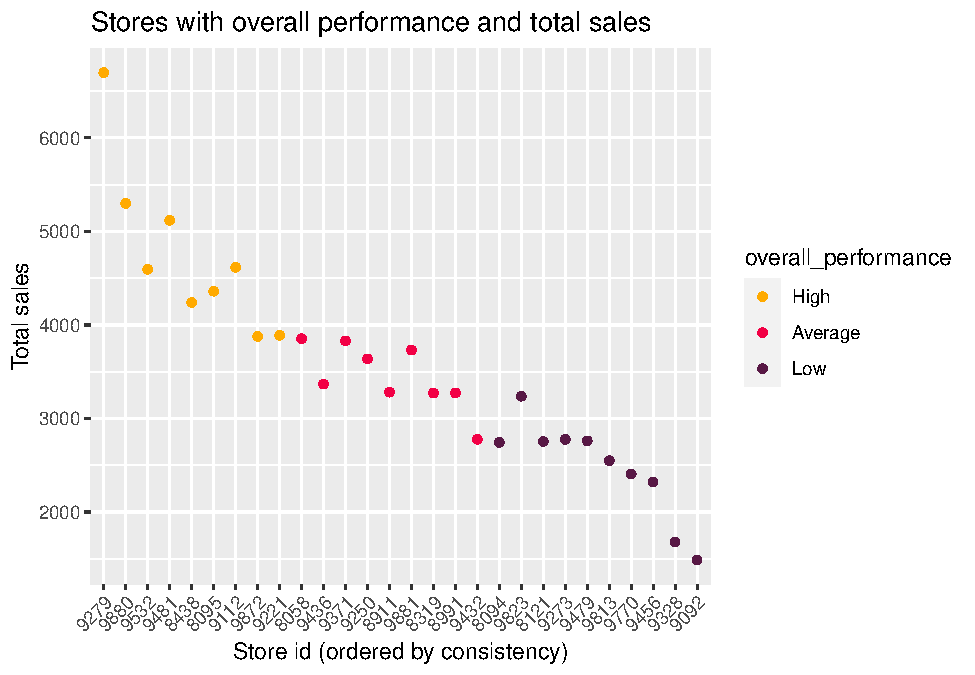
\includegraphics[width=0.75\linewidth]{Assignment-STAT702---final_files/figure-latex/new ranking-1}

Below is a plot showing that when a product is featured and/or displayed
weekly sales are more likely to be high. Weekly performance has been
categorised into `High', `Average' and `Low' based on the interquartile
range of weekly sales. When the product is featured and/or displayed a
higher proportion of weekly sales have been `High' or `Average' compared
to no promotion. Low performing stores could boost their sales by
increasing the number of weeks they promote the product and unreliable
stores could ensure high sales by holding regular promotions.

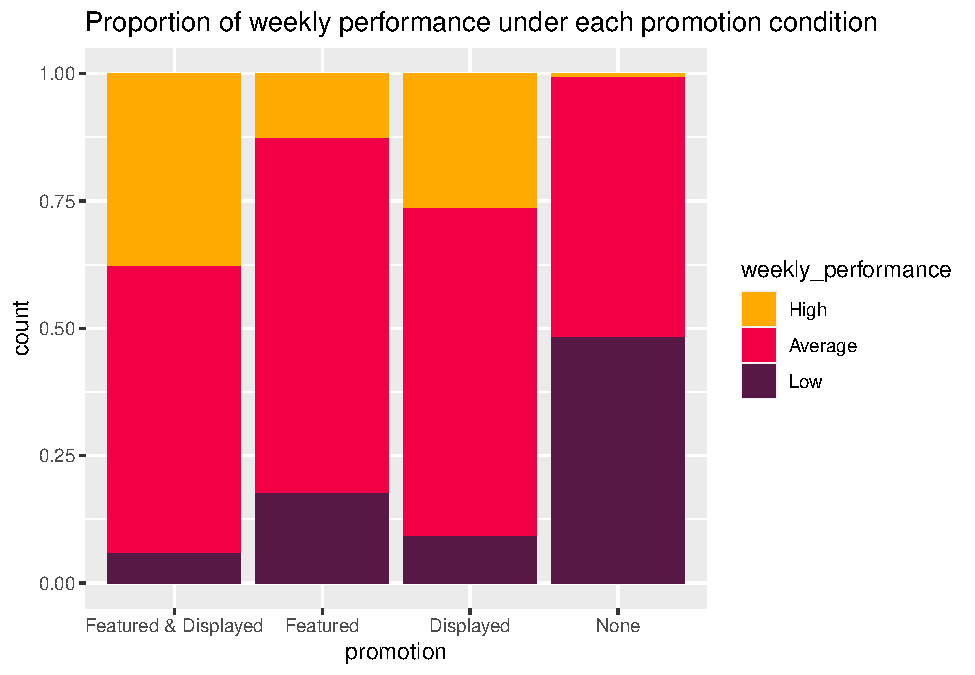
\includegraphics[width=0.5\linewidth]{Assignment-STAT702---final_files/figure-latex/1b promotion conditions-1}

\hypertarget{question-2}{%
\section{Question 2}\label{question-2}}

\hypertarget{a.i}{%
\subsection{2.a.i}\label{a.i}}

The Economic Order Quantity (EOQ) model is used to find the best order
quantity so that total costs are minimised. Key assumptions to this
model are that demand is constant and known, there is no lead time,
orders arrive instantaneously and back orders are not allowed. Another
assumption is that stock levels are under continuous review.

Demand for product 216233 has been estimated based on the annual demand
from 2012, this is 169591. The optimum order quantity is calculated
based on this demand and the annual order and holding costs. The
following EOQ formula is used to determine optimal order quantity where
k is order cost and h is holding cost.

\[Q^* =  \sqrt{\frac{2kA}{h}}\] The optimal order quantity is calculated
to be 5422 with an inventory cycle of 12 days. This means that every 12
days 5422 units are ordered, resulting in 31 annual orders. This model
results in the smallest possible annual inventory cost of 8132.6803762
with an annual order cost of 4066.1803762 and an annual holding cost of
4066.5. This EOQ model is plotted for two cycles below.

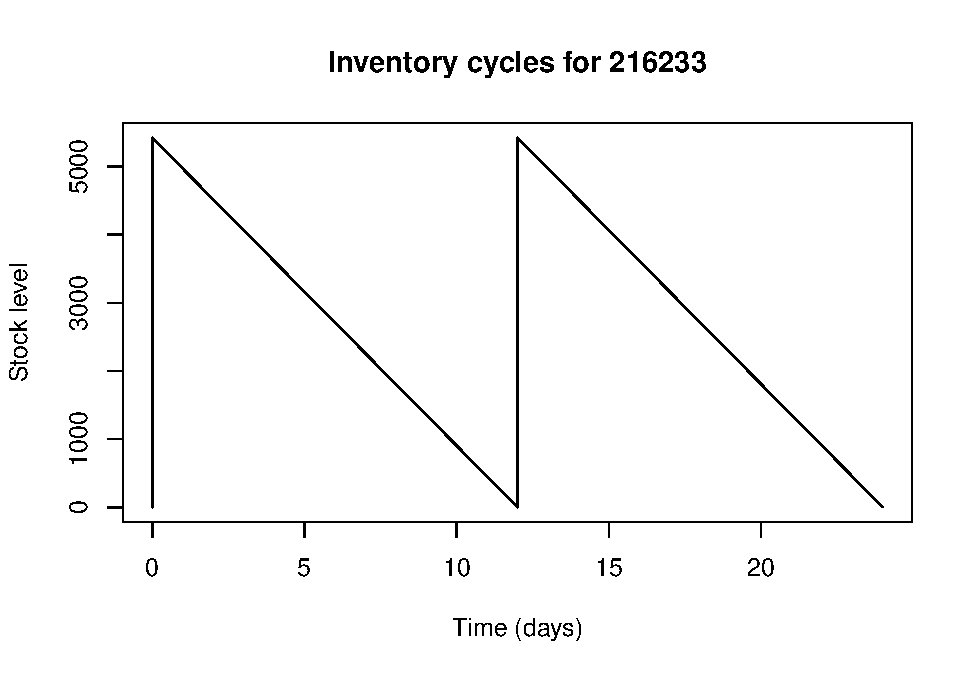
\includegraphics[width=0.75\linewidth]{Assignment-STAT702---final_files/figure-latex/2ai plot-1}

\hypertarget{a.ii}{%
\subsection{2.a.ii}\label{a.ii}}

The Optimum Backorder Model is used to find the best order quantity so
that total costs are minimised when backorders are allowed. Similar to
the EOQ model assumptions are made that demand is constant and known,
there is no lead time, orders arrive instantaneously and stock levels
are under continuous review.

Annual demand is estimated as 169591 using 2012 data. Backorders cost is
approximately 5\% of the total price per unit. In the 2012 sales data
total price for product 216233 varies from 78.4 to 134.7. For evaluating
the backorder cost the mean total price 78.4 has been used, resulting in
a backorder cost (p) of 6.22 per unit. The optimum quantity \((Q^*)\)
and optimum maximum inventory level \((S^*)\) are calculated using the
following forumlas.

\[Q^* = \sqrt{\frac{2kA}{h}} \sqrt{\frac{p+h}{p}} \]
\[S^* = \sqrt{\frac{2kA}{h}} \sqrt{\frac{p}{p+h}} \] Optimal order
quantity is calculated to be 6040 with an inventory cycle of 13 days.
This means that every 13 days 6040 units are ordered, resulting in 28
annual orders. The optimum inventory level is 4867 and the proportion of
time taking back orders is 23\%. This model results in the smallest
possible annual inventory cost of 7300.44 with an annual order cost of
3650.14 and an annual holding cost of 2941.35 and annual backorder cost
of 709. This EOQ model is plotted for two cycles below.

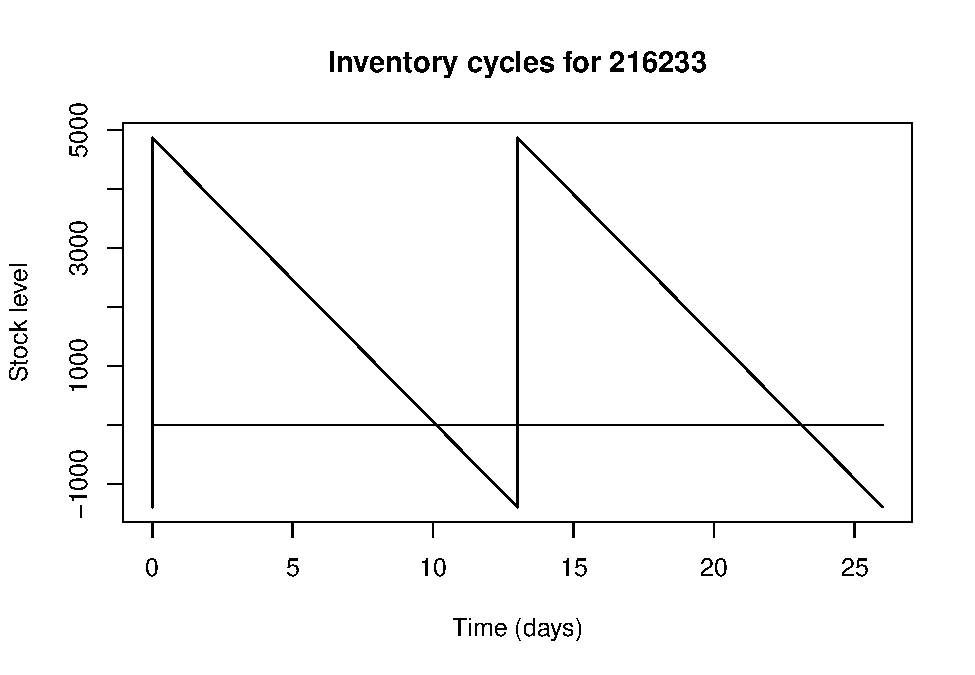
\includegraphics[width=0.75\linewidth]{Assignment-STAT702---final_files/figure-latex/2aii plot-1}

\hypertarget{a.iii}{%
\subsection{2.a.iii}\label{a.iii}}

The plot below shows the weekly demand from the 2012 sales data plotted
with the optimum order frequency, 13 days and optimum order quantity
6040 from the Optimum Backorder Model. Stock starts at the optimum
inventory level 4867, decreases with every weekly sale quantity from
2012 data and increases with inventory added at the optimum frequency
and quantity.

Actual demand is not constant and as a result the quantity and frequency
found with the back order model is not always appropriate. The model
performs best when demand is constant, for example in July.

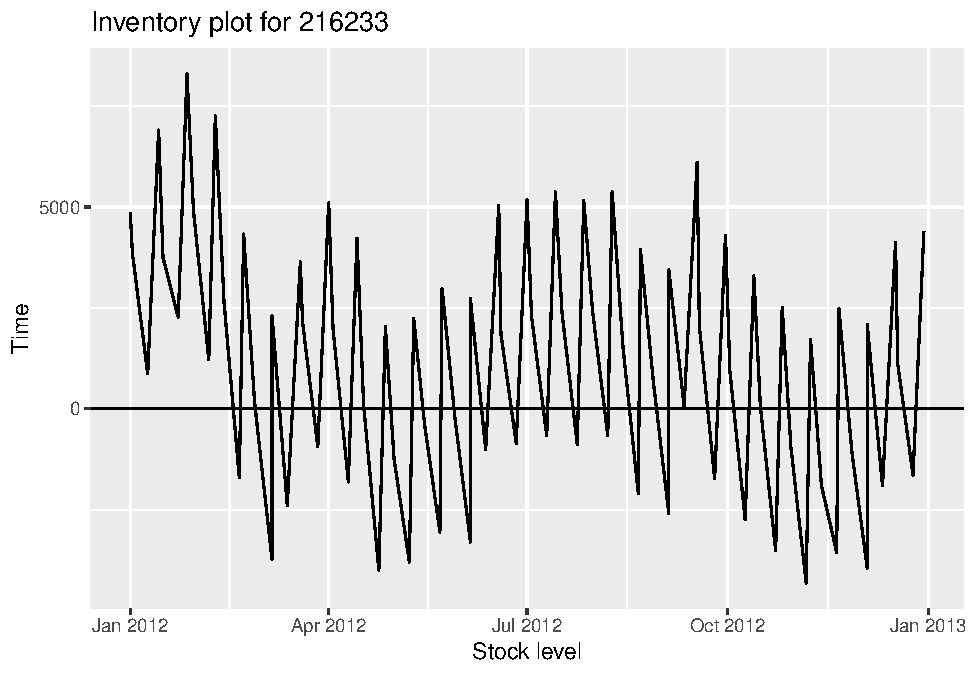
\includegraphics[width=0.75\linewidth]{Assignment-STAT702---final_files/figure-latex/2aiii-1}

\hypertarget{b.i.}{%
\subsection{2.b.i.}\label{b.i.}}

For this multi-inventory model demand during a one week lead time has
been estimated using the mean and standard deviation of observed data in
2012. Demand has been estimated as a normal distribution with a mean of
2057 and standard deviation of 523. As the plot below shows, whilst the
actual demand for 2012 does not perfectly follow this distribution it is
a adequate approximation.

The expected annual demand is estimated to be 106939. Given this annual
demand and the costs of holding and reordering stock, the recommended
multi-inventory model is to order 821 units whenever the order quantity
reaches the reorder point of 2916 units. Approximately 130 orders will
be placed per year and safety stock is 821. This approach ensures
roughly 95\% of the time stock will be sufficient for weekly demand. The
expected annual costs are 10926.75 per year. If demand was certain the
annual costs would only be 5338.47 so the additional cost of holding
safety stock is 5588.28.

\begin{verbatim}
## integer(0)
\end{verbatim}

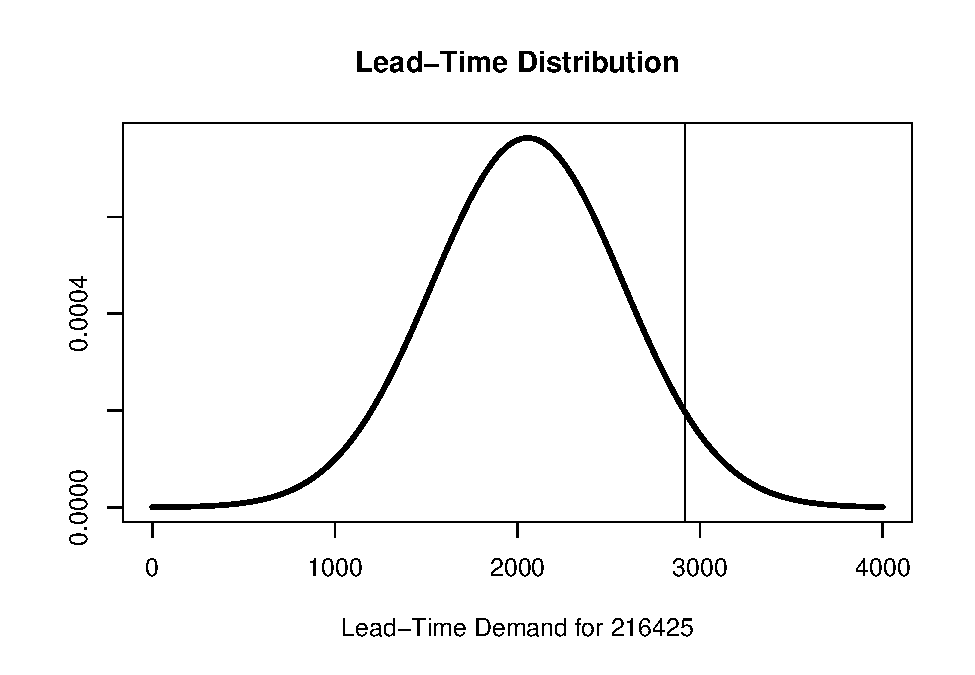
\includegraphics[width=0.5\linewidth]{Assignment-STAT702---final_files/figure-latex/2bi plots,figures-side-1}
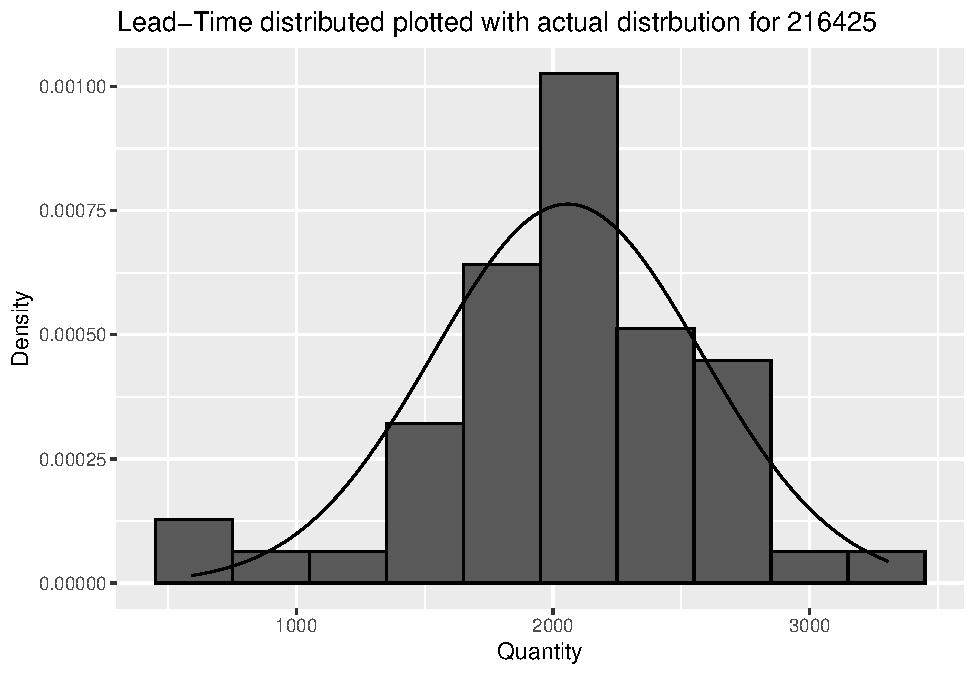
\includegraphics[width=0.5\linewidth]{Assignment-STAT702---final_files/figure-latex/2bi plots,figures-side-2}

\hypertarget{b.ii}{%
\subsection{2.b.ii}\label{b.ii}}

For this multi-inventory model, demand during a one week lead time has
been estimated using the mean and standard deviation of observed data in
2012. Demand has been estimated as a normal distribution with a mean of
739 and standard deviation of 410. As the plot below shows this
distribution is a very poor fit for the observed data. It is recommended
that a more accurate distribution is used for estimating the Lead-Time
distribution and reorder point. It is likely that the reorder point
calculated with this normal distribution is unnecessarily high.

The expected annual demand is estimated to be 38410. Given this annual
demand and the costs of holding and reordering stock, the recommended
multi-inventory model is to order 492 units whenever the order quantity
reaches the reorder point of 1413 units. Approximately 78 orders will be
placed per year and safety stock is 492. This approach ensures roughly
95\% of the time stock will be sufficient for weekly demand. The
expected annual costs are 7582.37 per year. If demand was certain the
annual costs would only be 3199.42 so the additional cost of holding
safety stock is 4382.95.

\begin{verbatim}
## integer(0)
\end{verbatim}

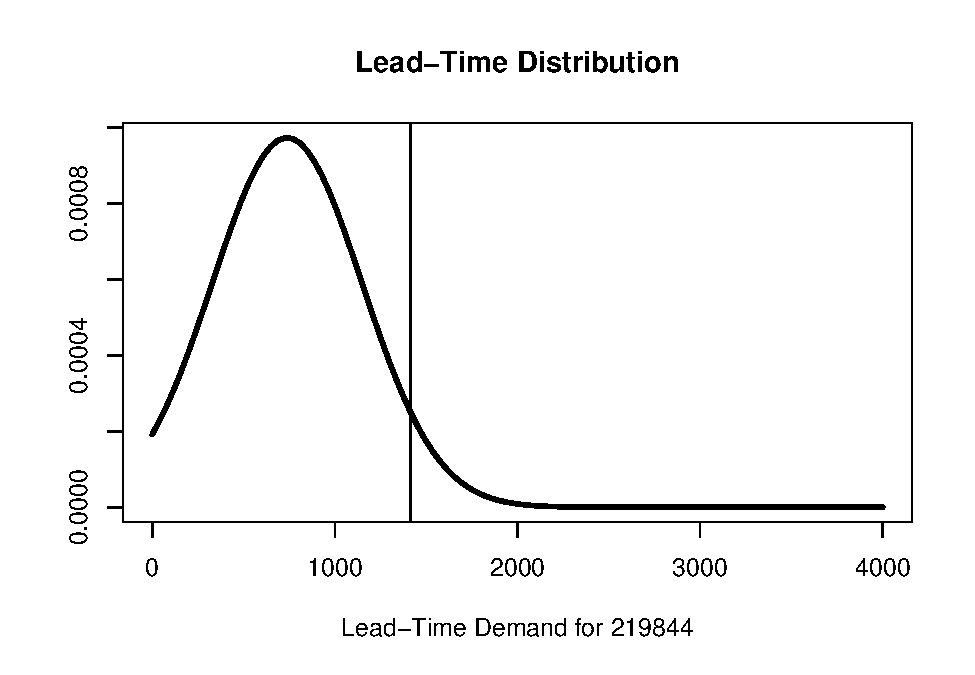
\includegraphics[width=0.5\linewidth]{Assignment-STAT702---final_files/figure-latex/2bii lead-time distribution plot, figures-side-1}
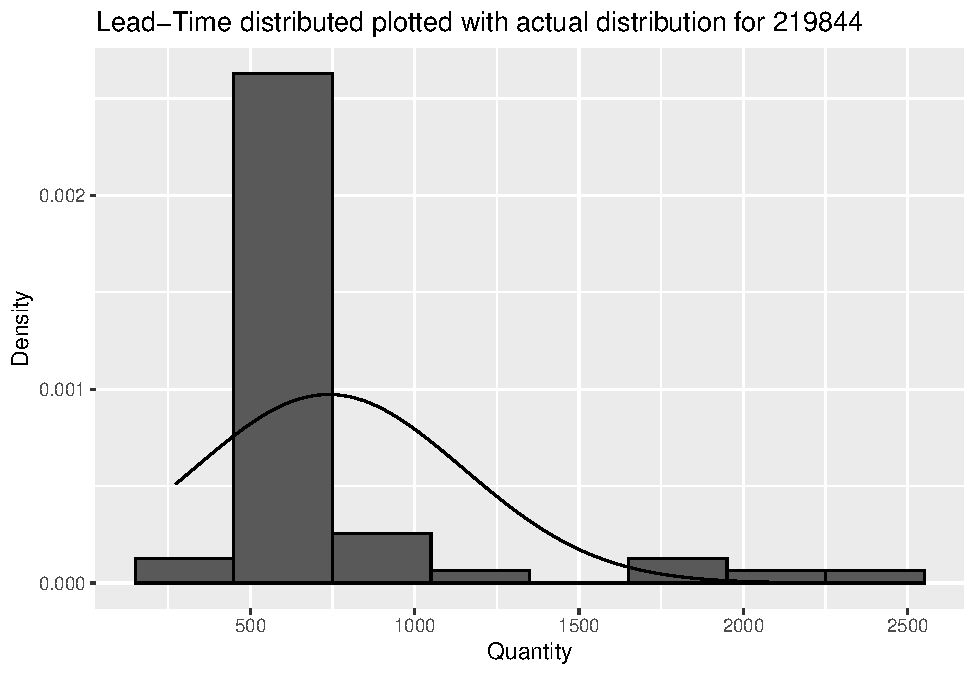
\includegraphics[width=0.5\linewidth]{Assignment-STAT702---final_files/figure-latex/2bii lead-time distribution plot, figures-side-2}

\begin{verbatim}
## integer(0)
\end{verbatim}

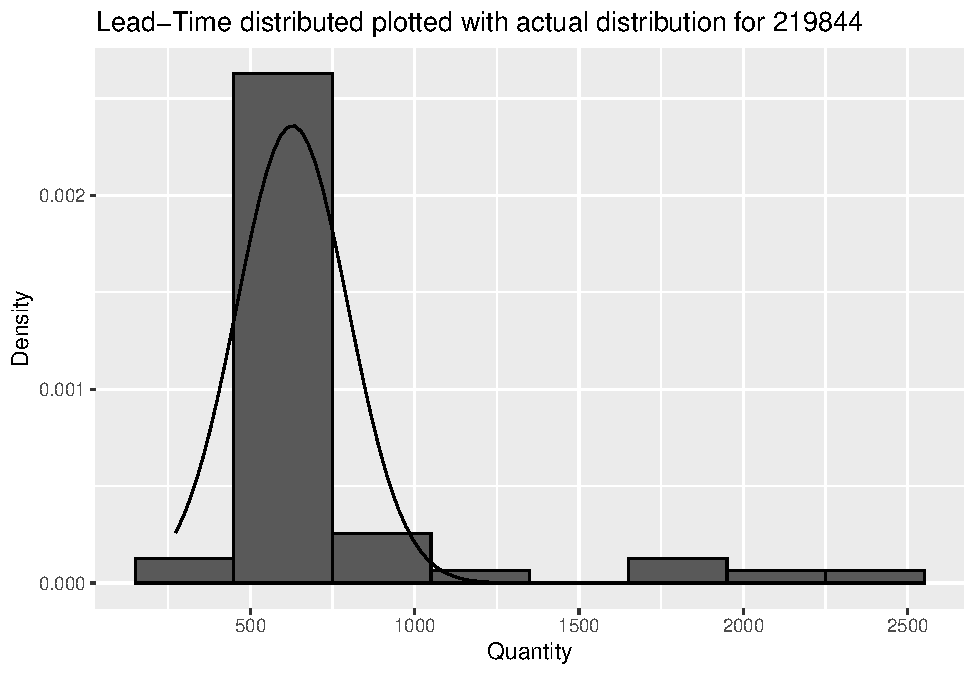
\includegraphics[width=0.5\linewidth]{Assignment-STAT702---final_files/figure-latex/actual distribution plot, figures-side-1}
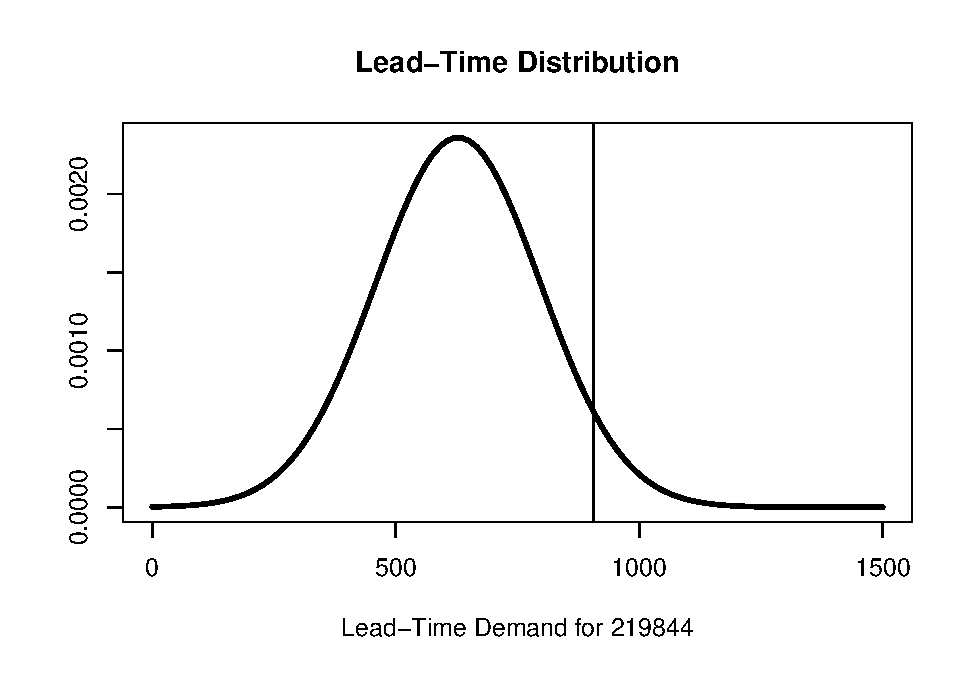
\includegraphics[width=0.5\linewidth]{Assignment-STAT702---final_files/figure-latex/actual distribution plot, figures-side-2}

\hypertarget{question-3}{%
\section{Question 3}\label{question-3}}

\hypertarget{a-1}{%
\subsection{3.a}\label{a-1}}

Reviews were rated from 1-5. The mean rating for product B00006IE7J is
4.7. Most reviews were rated highly with 79\% given 5 stars and 13.4\%
given 4 stars.

\begin{longtable}[]{@{}llllll@{}}
\toprule
Min & 1st Qu. & Median & Mean & 3rd Qu. & Max \\
\midrule
\endhead
1 & 5 & 5 & 4.7 & 5 & 5 \\
\bottomrule
\end{longtable}

Some reviews were verified and others were not. The proportion of
ratings given by these different groups are compared below. The
unverified group gave a higher proportion of ratings 2-4 than the
verified group.

Review ratings have been plotted below against time. Most reviews were
given between 2014 and 2018. Rating does not appear to be strongly
correlated with time.

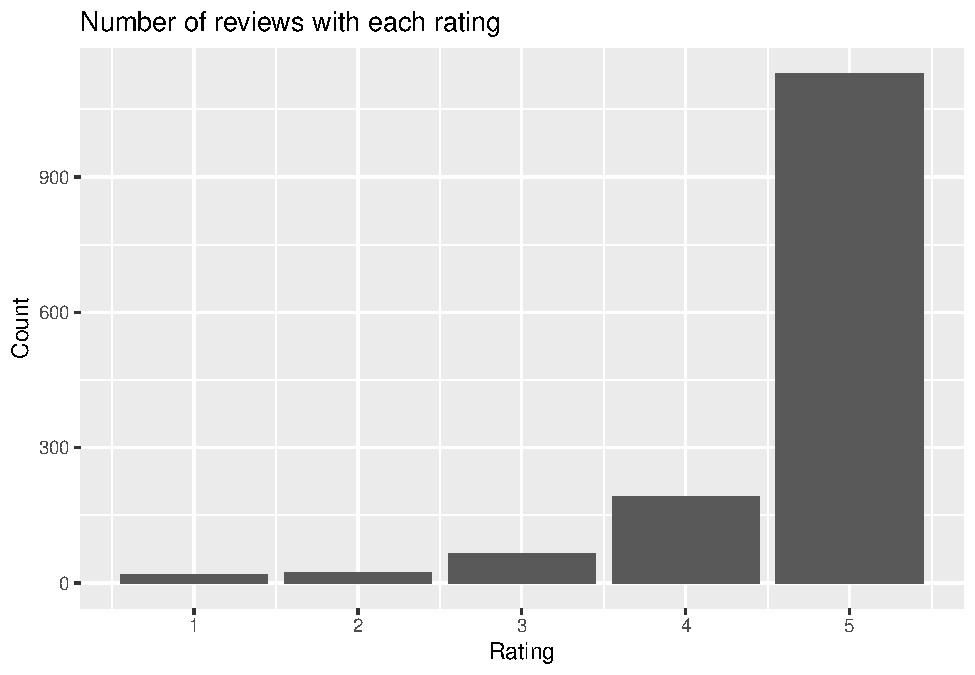
\includegraphics[width=0.5\linewidth]{Assignment-STAT702---final_files/figure-latex/3a plots-1}
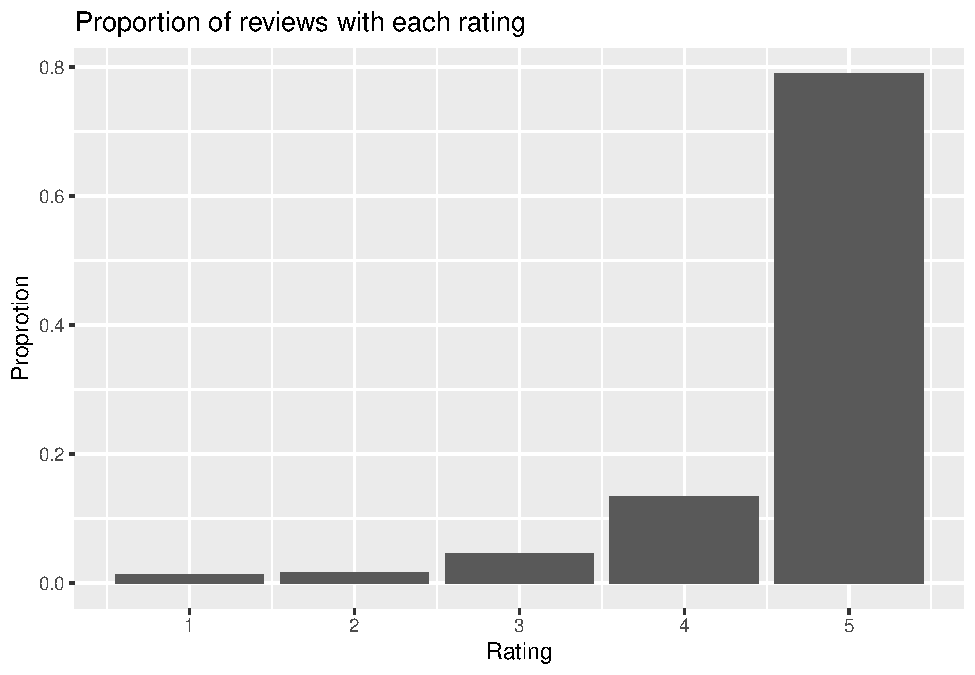
\includegraphics[width=0.5\linewidth]{Assignment-STAT702---final_files/figure-latex/3a plots-2}
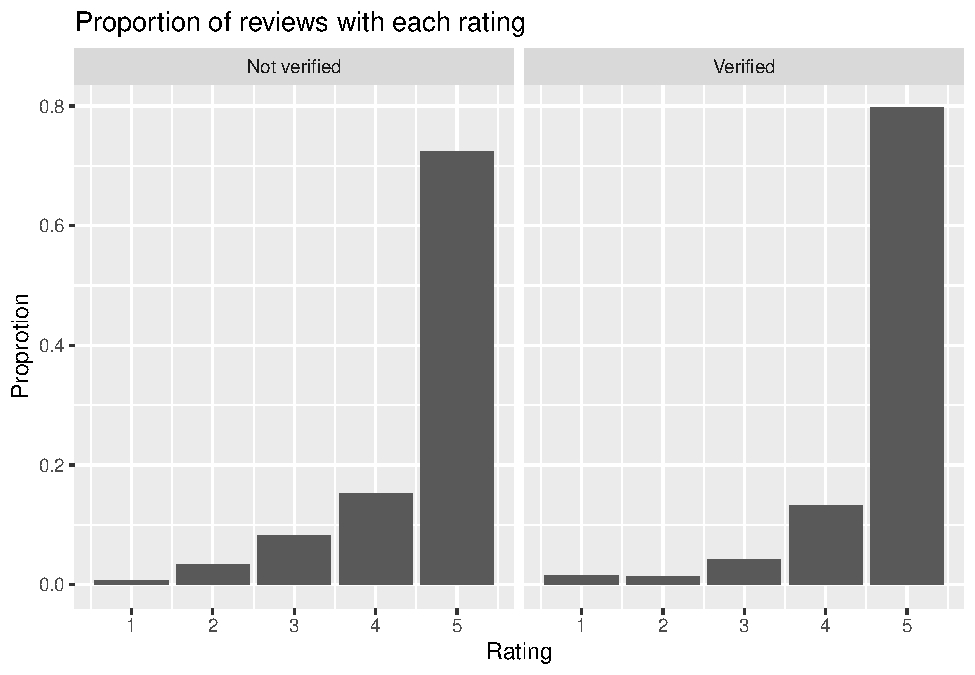
\includegraphics[width=0.5\linewidth]{Assignment-STAT702---final_files/figure-latex/3a plots-3}
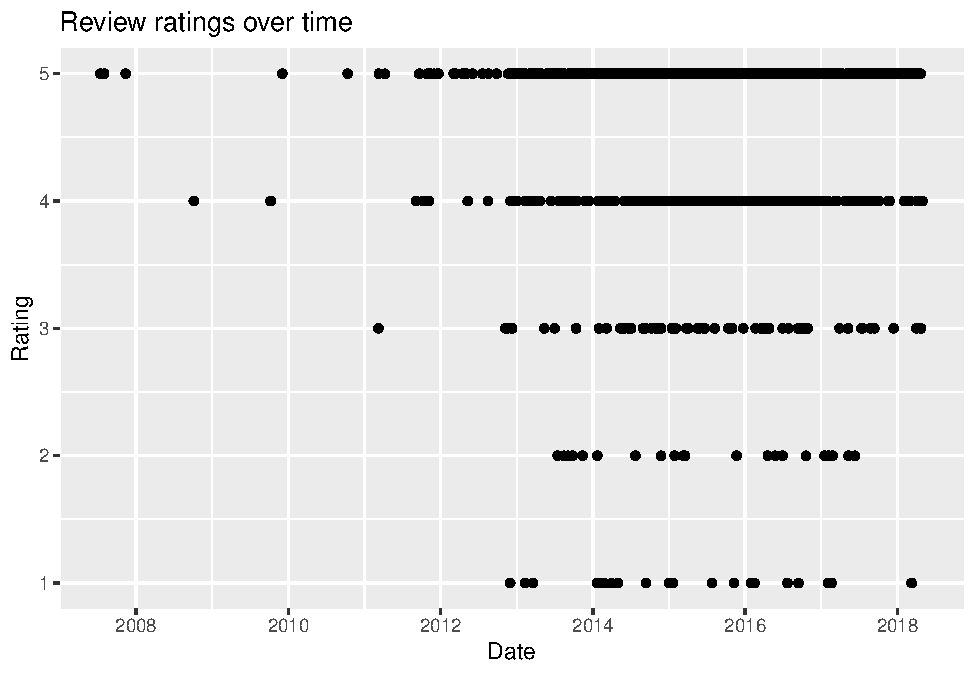
\includegraphics[width=0.5\linewidth]{Assignment-STAT702---final_files/figure-latex/3a plots-4}

\hypertarget{b-1}{%
\subsection{3b}\label{b-1}}

Review text has been tokenised and stop words have been removed. Stop
words are words such as `the' and `it' that hold little information for
sentiment analysis. The top 10 words in reviews are plotted below along
with their frequency.

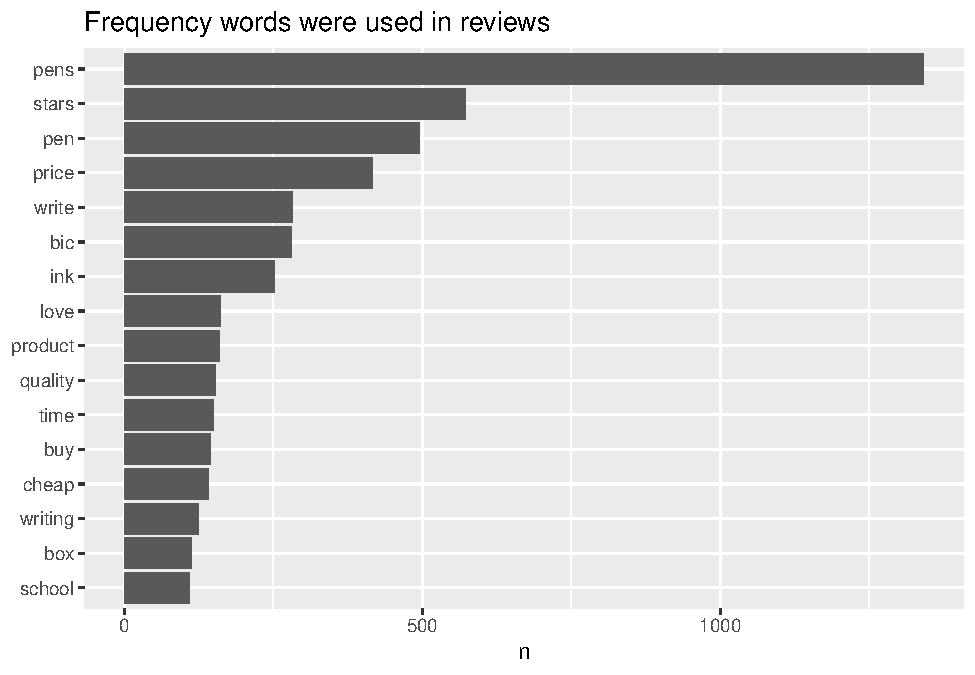
\includegraphics[width=0.5\linewidth]{Assignment-STAT702---final_files/figure-latex/3b word frequency-1}

In the plot above we can see a few words that can be considered as stop
words. Words like \texttt{pen} and \texttt{stars} are not very valuable
to the sentiment. These words are removed from the data set as well.

Notably the top words are `pens', `stars' and `pen'. The product that is
being analysed is bic pens, this explains why these words occur
frequently. Users provide a 5 star rating, in their review users then
refer to their rating and this explains why the word `stars' occurs
frequently. These words offer little information about how reviewers
feel about the product so these are removed from reviews for the next
part of analysis.

The remaining words are given a sentiment rating, high ratings indicate
positive sentiment and low ratings indicate negative sentiment. The top
10 frequently used negative and positive words are presented below along
with a word cloud of the top 100 words.

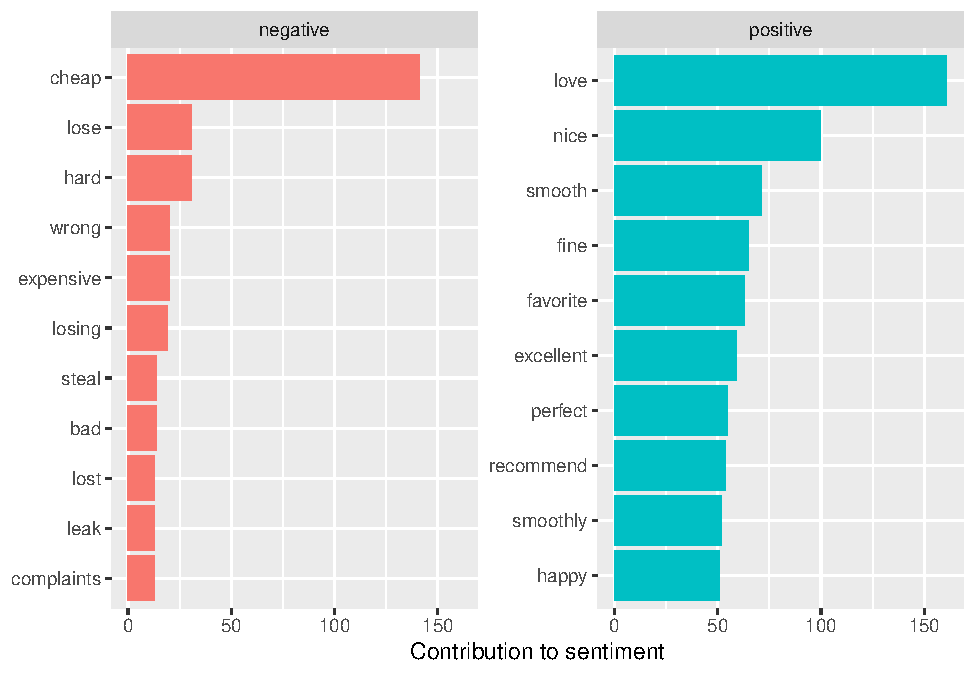
\includegraphics[width=0.75\linewidth]{Assignment-STAT702---final_files/figure-latex/3b word sentiment-1}

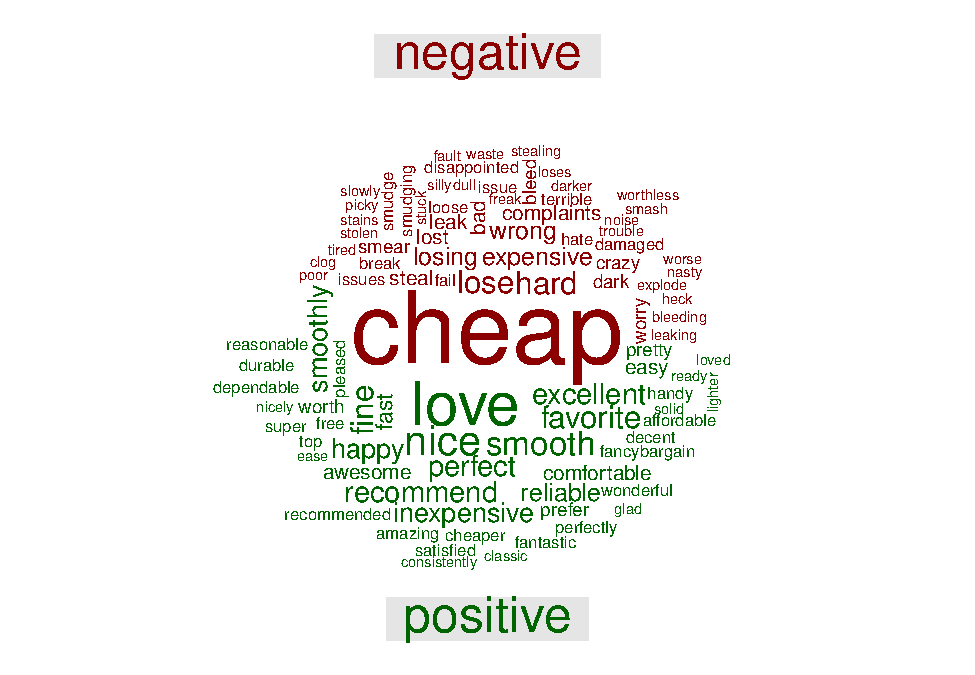
\includegraphics[width=0.75\linewidth]{Assignment-STAT702---final_files/figure-latex/3b word cloud-1}

Notably the word `cheap' is the most commonly used negative word and is
used significantly more frequently than any other negative word. `Cheap'
can be used to say something is low quality, however in the context of a
pen `cheap' is likely to be a positive descriptor as people often don't
want to spend too much money on pens. Overall 141 reviews included the
word `cheap', 0.7446809\% were 5 star reviews and 0.1560284\% were 4
star reviews. This indicates that `cheap' is more likely to indicate a
positive rather than negative sentiment.

For each review the word sentiments are added together giving the review
an overall sentiment score. Below is a plot showing the proportion of
reviews in each rating category were given an overall negative or
positive sentiment rating. When the word `cheap' is excluded there is a
small change with a decreased proportion of 3-5 ratings classified as
negative. This indicates better performance classification.

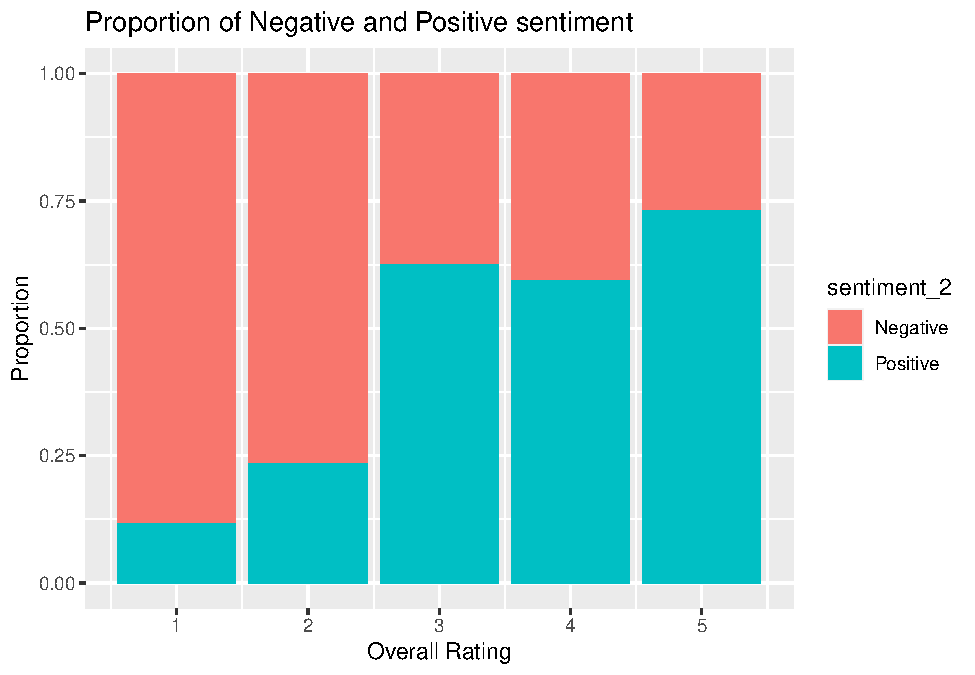
\includegraphics[width=0.5\linewidth]{Assignment-STAT702---final_files/figure-latex/3b comparison,figures-side-1}
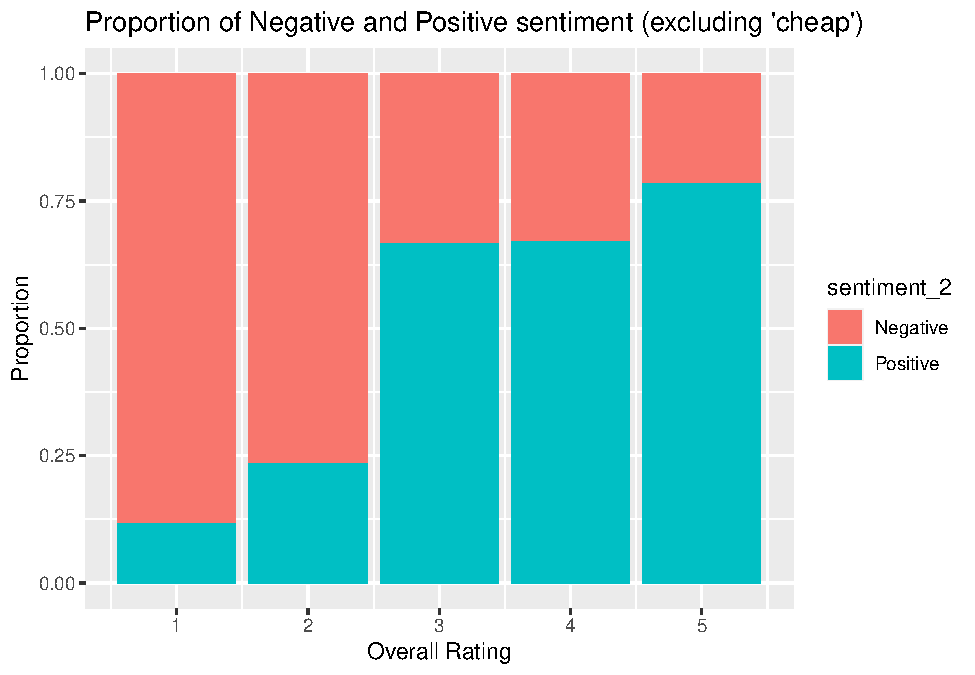
\includegraphics[width=0.5\linewidth]{Assignment-STAT702---final_files/figure-latex/3b comparison,figures-side-2}
The graphs below plot the top 100 negative and top 100 positive
sentiment values against the actual overall values specified by the
reviewers. In the positive reviews, majority of the data is classified
as an overall rating of 3 or above. A single outlier exists. The outlier
has an overall value of 1 and a positive sentiment associated to it. In
the negative reviews, an outlier can be seen, where the overall rating
is 5 but the sentiment given to the data is very negative. Additionally,
a lot of data rated 5 stars has been given a negative sentiment. This
can be attributed to the data not being balanced or the reviews having
too many words. Both can affect the final analysis in different ways and
must be considered as a way to improve sentiment analysis on the given
data.

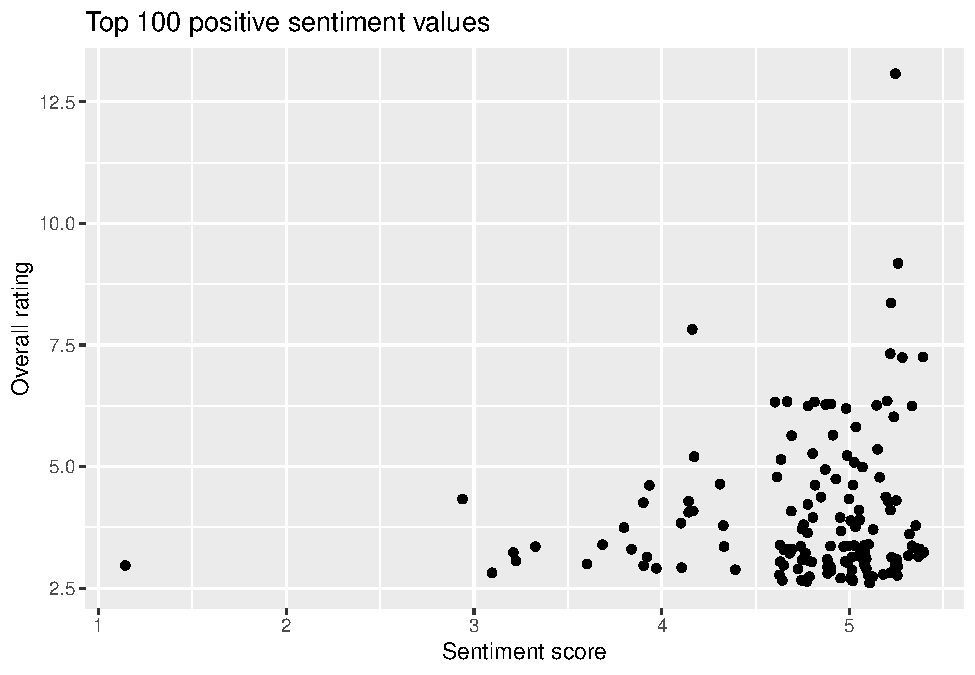
\includegraphics[width=0.5\linewidth]{Assignment-STAT702---final_files/figure-latex/top positive and negative sentiment scores, figures-side-1}
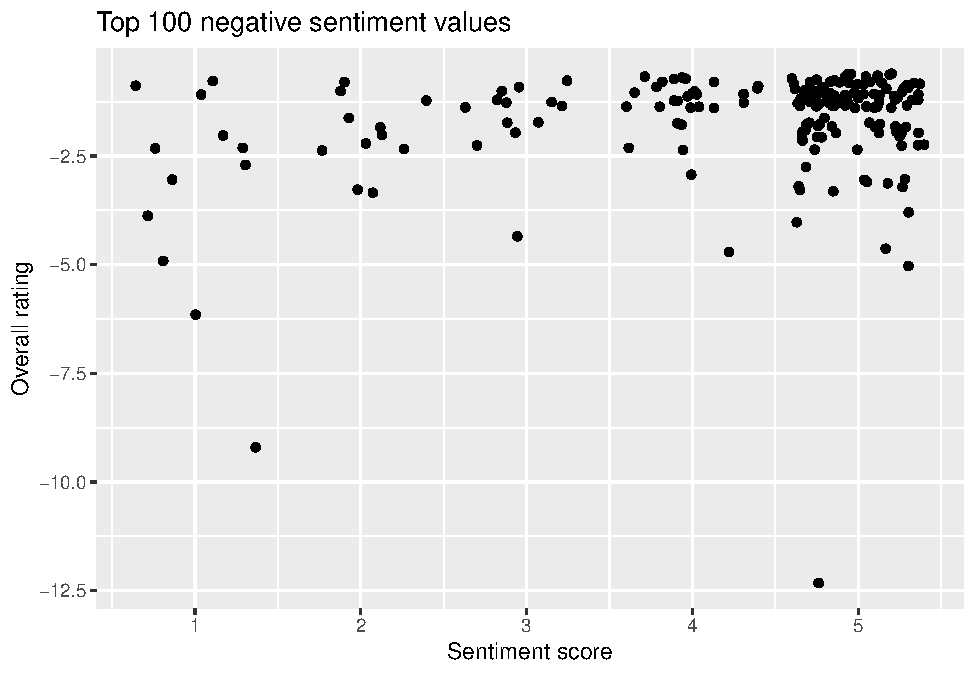
\includegraphics[width=0.5\linewidth]{Assignment-STAT702---final_files/figure-latex/top positive and negative sentiment scores, figures-side-2}
\newpage

\hypertarget{appendix-a} I contributed by solving question 1 and 3 in this
project. I also compared my answers to my partner's question1 answers to
make sure we had done the right thing. I initially tackled question 3
and asked Genevieve to help me out with beautifying some of the plots. I
was happy to brainstorm solutions and ideas with my partner on anything
we worked on. Finally, I was able to help add attention to detail with
the final formatting of our document.

\textbf{Genevieve 60\%}

\end{document}
